\section{Related work}
There are several existing HDI visualization tools that allow user to view the dataset in a non-interactive way. UNDP has a line chart as shown in Figure \ref{fig:undp}. The x axis is the year, and the y axis is the HDI value.  Each line represents one country that users can hover on to see the HDI value. It can be convenient if the users can view the common trend for all the countries or if the users can find a country with the highest or lowest HDI value for a given year. However, there is no much information they can retrieve from the middle range of data where many lines congest together. Also, it can be hard for the users to select a country. Another major visualization for HDI is Visualizing Human Development Index 2013 from Amazon AWS as shown in Figure \ref{fig:amazon} that provides four line charts for HDI components and a color map showing different HDI values. Users are able to hover on the map or the line to see the corresponding country highlighted. It also includes a population chart for viewing how the population is distributed among different HDI values.  The comparison view between the map and the graphs provides more information than the single line chart from UNDP. However, it did not provide any filtering functionality if the users only want to view countries with high HDI. And it can be hard to find a country as well if the user does not know where the country is located on the map. For our visualization, we will try to provide users more functionality to interact with the visualization so that they can easily find information they need.
\begin{figure}[t]
	\centering
	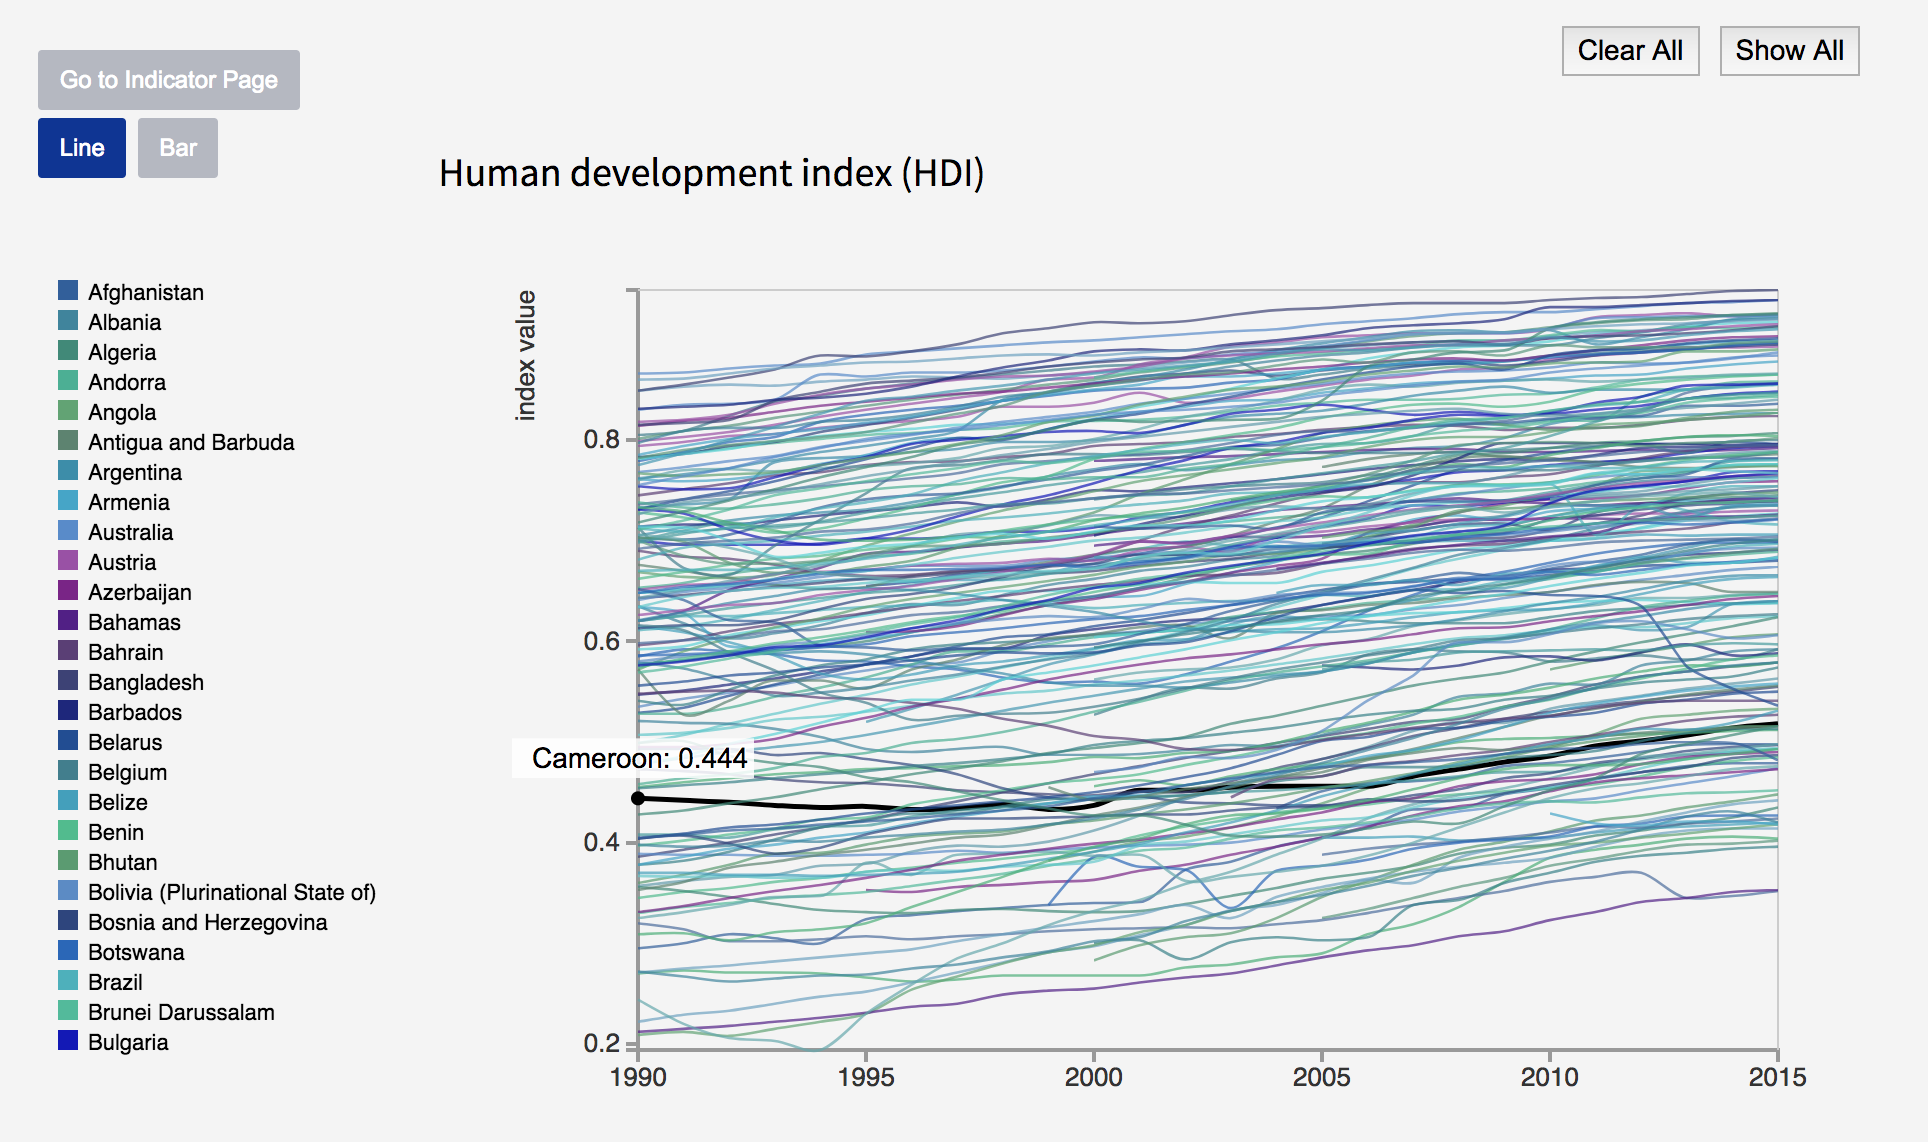
\includegraphics[width=0.4\textwidth]{undp}
	\caption{Line chart map from UNDP}
	\label{fig:undp}
\end{figure}
\begin{figure}[t]
	\centering
	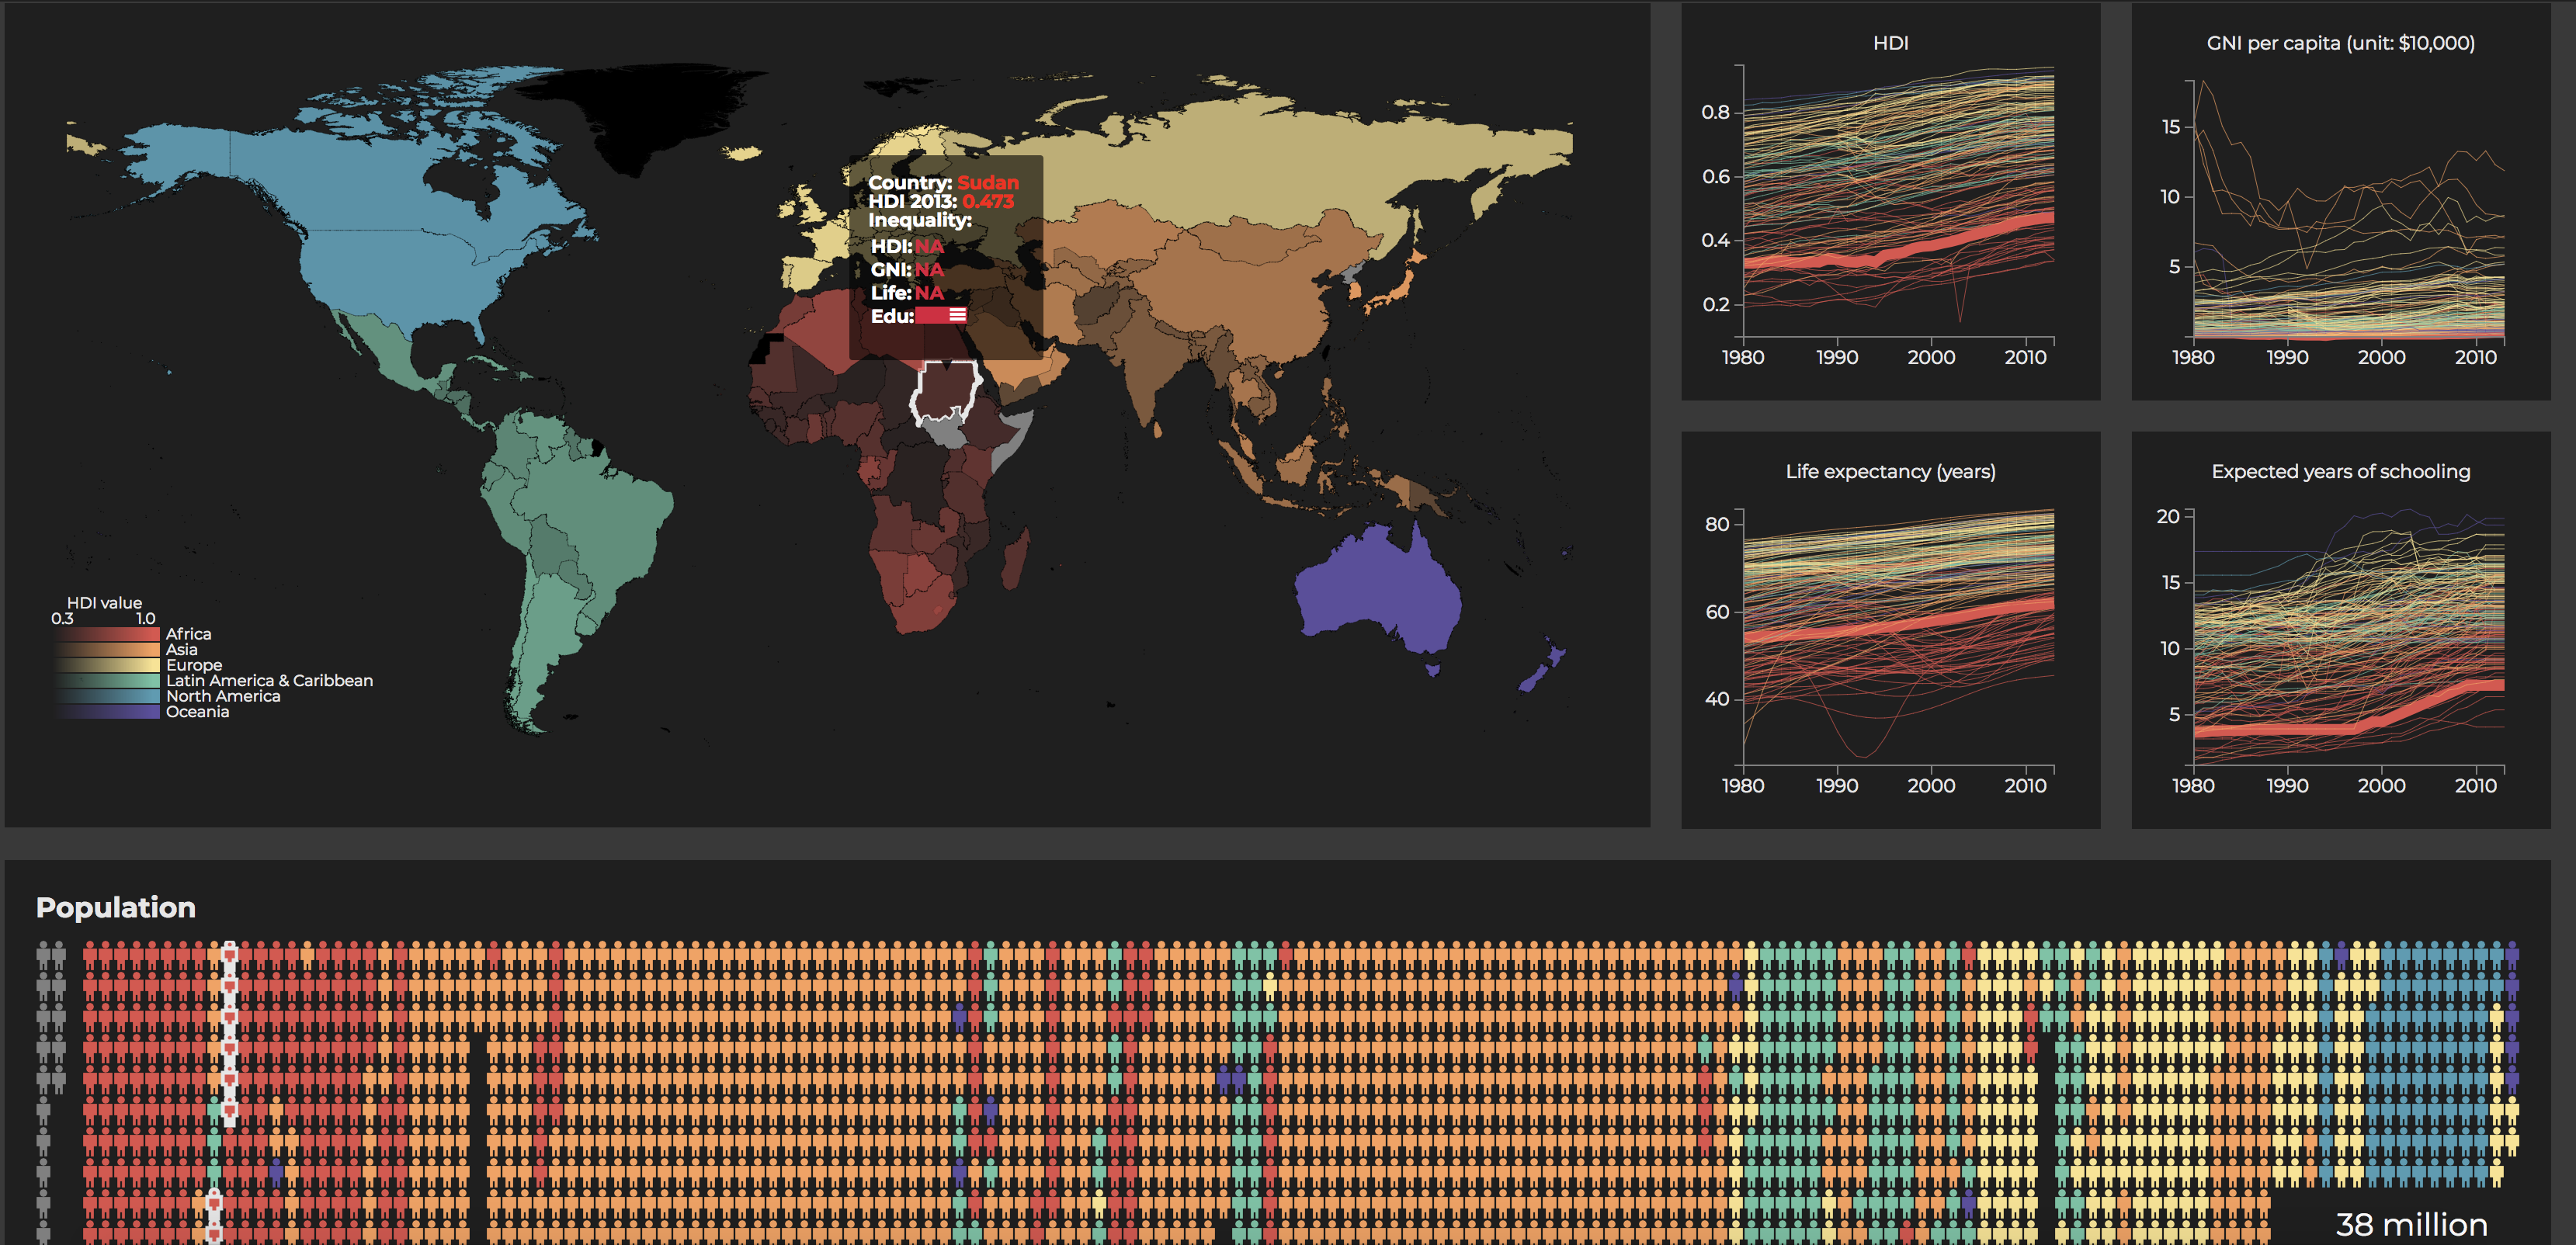
\includegraphics[width=0.4\textwidth]{amazon}
	\caption{Visualizing Human Development Index 2013}
	\label{fig:amazon}
\end{figure}
